\documentclass[10pt,letterpaper]{article}
\usepackage[margin=1in]{geometry}
\usepackage{graphicx}
\usepackage{amsmath,amssymb,amsthm}
\usepackage{enumerate}
\usepackage{tikz}
\usepackage{xcolor}
\usepackage{hyperref}
\usepackage[numbers]{natbib}
\usepackage[ruled]{algorithm2e}

\setlength\parindent{0pt}
\renewcommand\qedsymbol{$\blacksquare$}
\theoremstyle{definition}
\newtheorem{theorem}{Theorem}[section]
\newtheorem{corollary}[theorem]{Corollary}
\newtheorem{lemma}[theorem]{Lemma}
\newtheorem{definition}[theorem]{Definition}
\newtheorem{example}[theorem]{Example}
\theoremstyle{remark}
\newtheorem*{remark}{Remark}

\title{Lecture: Lagrange Duality\footnote{Some of this material is based on Boyd and Vandenberghe's seminal text \emph{Convex Optimization}. If you'd like more details see that book. It's freely available online.}}
\author{Conner DiPaolo\thanks{Harvey Mudd College (\url{cdipaolo@hmc.edu})}}
\date{Monday, December 3, 2018}

\newcommand\inner[1]{\langle #1 \rangle}
\newcommand\R{\mathbb{R}}
\newcommand\C{\mathbb{C}}
\newcommand\M{\mathsf{M}}
\renewcommand\P{\mathbf{P}}
\newcommand\E{\mathbf{E}}
\renewcommand\O{\mathcal{O}}
\newcommand\Var{\mathbf{Var}}
\newcommand\tr{\operatorname{tr}}
\newcommand\N{\mathcal{N}}
\newcommand\m[1]{\begin{bmatrix} #1 \end{bmatrix}}

\newcommand\A{\boldsymbol{A}}
\newcommand\Q{\boldsymbol{Q}}
\newcommand\U{\boldsymbol{U}}
\renewcommand\L{\boldsymbol{\Lambda}}
\renewcommand\S{\boldsymbol{\Sigma}}
\newcommand\I{\boldsymbol{I}}
\newcommand\x{\boldsymbol{x}}
\newcommand\z{\boldsymbol{z}}
\newcommand\g{\boldsymbol{g}}
\renewcommand\r{\boldsymbol{r}}
\newcommand\e{\boldsymbol{e}}
\newcommand\lambdab{\boldsymbol{\lambda}}
\newcommand\nub{\boldsymbol{\nu}}
\renewcommand\c{\boldsymbol{c}}
\renewcommand\a{\boldsymbol{a}}
\renewcommand\b{\boldsymbol{b}}

\begin{document}

\maketitle

%%%%%%%%%%%%%%%%%%%%%%%%%%%%%%%%%%%%%%%%%%%%%%%%%%%%%%%%%%%%%%%%
%%%                       Part 1                             %%%
%%%%%%%%%%%%%%%%%%%%%%%%%%%%%%%%%%%%%%%%%%%%%%%%%%%%%%%%%%%%%%%%
\section{Lagrange Duality in Optimization}

Lagrange duality allows us to turn one constrained optimization problem (called the \emph{primal problem}) into another constrained optimization (called the \emph{dual problem}) which is intimately related. In many cases of interest, the problems are equivalent to each other in that their optimal values are equal, and that solving one allows us to solve the other problem easily. This provides flexibility to the optimizer, since it allows her to choose between
\begin{enumerate}[(a)]
    \item solving the primal problem by itself,
    \item solving the dual problem by itself, or
    \item solving each problem together,
\end{enumerate}
depending on which approach provides the most computationally efficient solution. We've seen the gradient descent algorithm for solving convex optimization problems already (an example of (a)), but there are other algorithms (like the mirror descent algorithm) which exploit (b) to solve the primal problem. We'll see an example later where solving the primal and dual problem \emph{jointly} allows us to solve explicitly linearly constrained convex quadratic programs in a computationally efficient way.

\subsection{Generic Optimization Problems}

A generic optimization problem can be framed in the following way:
\begin{align*}
    \text{minimize: } & f_0(\x)\\
    \text{subj. to: } & f_i(\x) \leq 0,\quad i=1,\ldots,m\\
                      & h_i(\x) = 0,\quad i=1,\ldots,p,
\end{align*}
where $\x$ varies over $\R^n$. This will be called the primal problem, and it's
optimal value will be denoted $p^\star$ (following [BoydVandenberghe]).

\begin{example}
    Consider the optimization problem
    \begin{align*}
        \text{maximize: } & \c^*\x\\
        \text{subj. to: } & \A\x \leq \b\\
                          & \x\text{ has integer components.}
    \end{align*}
    where $\c\in\R^n$, $\b\in\R^m$, and $\A\in\R^{m\times n}$. This is
    a generic \emph{integer program}, and is NP-hard. We'll form this in the
    standard form given above. Note that $x\in\R$ is integral if and only if
    $\sin(\pi x) = 0$. Moreover, the constraint $\A\x \leq \b$ can be broken into the
    row constraints $\a_i^*\x \leq \b_i$ for all the rows $\a_i$ of $\A$. Thus this
    problem above is equivalent (in terms of optimal value and the actual minimizer $\x^\star$)
    to
    \begin{align*}
        \text{minimize: } & \c^*\x\\
        \text{subj. to: } & \a_i^*\x - \b_i \leq 0,\quad i=1,\ldots,m\\
                          & \sin(\pi x) = 0.
    \end{align*}
\end{example}

\subsection{The Dual Problem}

We'll start with some definitions. We'll let $I_\leq :\R\to \{0,\infty\}$ and $I_0 :\R \to \{0,\infty\}$
be the indicator functions of the non-positive reals and the point zero, respectively. That is,
\[
    I_\leq(x) = \begin{cases}
        0 & \text{if }x\leq 0\\
        \infty & \text{otherwise.}
    \end{cases},\qquad I_0(x) = \begin{cases}
        0 & \text{if }x=0\\
        \infty & \text{otherwise.}
    \end{cases}
\]

\begin{center}
    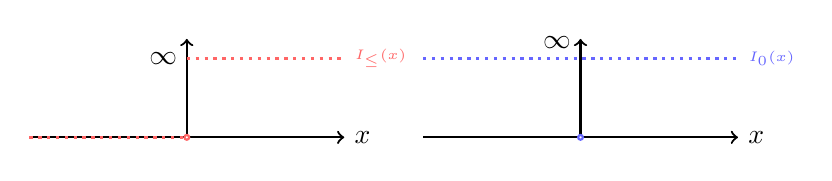
\begin{tikzpicture}
        \begin{scope}[shift={(-2.5,0)}]
            \draw[thick,->] (-2,0) -- (2,0) node[right] {$x$};
            \draw[thick,->] (0,0) -- (0,1.25);
            \node[left] at (0,1) {$\infty$};
            \draw[very thick,red!60,dotted] (-2,0) -- (0,0);
            \draw[very thick,red!60,dotted] (0,1) -- (2,1) node[right] {\tiny$I_\leq(x)$};
            \draw[red!60,fill=white,thick] (0,0) circle (0.03);
        \end{scope}
        \begin{scope}[shift={(2.5,0)}]
            \draw[thick,->] (-2,0) -- (2,0) node[right] {$x$};
            \draw[thick,->] (0,0) -- (0,1.25);
            \node[left] at (0,1.2) {$\infty$};
            \draw[very thick,blue!60,dotted] (-2,1) -- (2,1) node[right] {\tiny$I_0(x)$};
            \draw[blue!60,fill=white,thick] (0,0) circle (0.03);
        \end{scope}
    \end{tikzpicture}
\end{center}

Now let's give a variational characterization of these indicators (verify this!):
\[
    I_\leq(x) = \sup_{\lambda \geq 0} \lambda x,\qquad I_0(x) = \sup_{\nu\in\R} \nu x
\]
Observe what this means for optimization, however. Our original constrained optimization
problem is equivalent to
\begin{align*}
    p^\star &= \inf_{\x} f_0(\x) + \sum_{i=1}^m I_\leq(f_i(\x)) + \sum_{i=1}^p I_0(h_i(\x))\\
    &= \inf_{\x}\sup_{\substack{\lambdab\geq 0\\\nub\lessgtr 0}} \underbrace{f_0(\x) + \sum_{i=1}^m \lambdab_i f_i(\x) + \sum_{i=1}^p \nub_i h_i(\x)}_\text{called the Lagrangian $L(\x,\lambdab,\nub)$}.
\end{align*}
Thus
\[
    p^\star = \inf_{\x}\sup_{\substack{\lambdab\geq 0\\\nub\lessgtr 0}} L(\x,\lambdab,\nub),
\]
which is just a representation where the inner supremum ensures that $\x$ must lie in the contstraint
set, at which point we minimize over out objective in $\x$.\\

One might ask, what if we re-arranged the optimization procedure this gives us? That is,
instead of minimizing over $\x$ after maximizing over the \emph{Lagrange multipliers} $\lambdab$
and $\nub$, we first minimize over $\x$, giving the \emph{dual function}
\[
    g(\lambdab,\nub) = \inf_{\x}L(\x,\lambdab,\nub)
\]
before performing the maximization over $\lambdab$ and $\nub$
\[
    d^\star = \sup_{\substack{\lambdab\geq 0\\\nub\lessgtr 0}} g(\lambdab,\nub) = \sup_{\substack{\lambdab\geq 0\\\nub\lessgtr 0}}\inf_{\x} L(\x,\lambdab,\nub).
\]
As the notation suggests, the maximization problem giving us $d^\star$ is called the \emph{dual problem}
of the primal optimization giving $p^\star$. Notationally, this dual problem \emph{looks} intimately related
to the primal problem, but we can show a strong result, namely that the solution to the dual problem
allows us to bound the primal problem.

\begin{theorem}
    For any $\lambdab \geq 0$ and $\nub\in\R^p$, $$g(\lambdab,\nub) \leq p^\star.$$ In particular,
    $$d^\star = \sup_{\substack{\lambdab \geq 0\\\nub\lessgtr 0}}g(\lambdab,\nub) \leq p^\star.$$
\end{theorem}
\begin{proof}
    Note that for any $\lambdab\geq 0$ and $\nub\in\R^p$, if we consider a fixed $\x\in\R^n$,
    \[
        L(\x,\lambdab,\nub) \leq \sup_{\substack{\lambdab\geq 0\\\nub\lessgtr 0}} L(\x,\lambdab,\nub)
    \]
    Taking the infimum of both sides with respect to $\x$ gives
    \[
        g(\lambdab,\nub) = \inf_{\x} L(\x,\lambdab,\nub) \leq \inf_{\x} \sup_{\substack{\lambdab\geq 0\\\nub\lessgtr 0}} L(\x,\lambdab,\nub) = p^\star.
    \]
\end{proof}

\begin{example}
    Consider the optimization problem
    \begin{align*}
        \text{minimize: } & (x-1)^2\\
        \text{subj. to: } & x^2 \geq 4
    \end{align*}
    over the real line. Clearly the optimal $x^\star = 2$, with the associated $p^\star = (x^\star - 1)^2
    = 1$. This problem has Lagrangian
    \[
        L(x,\lambda) = (x-1)^2 + \lambda (4-x^2) = (1-\lambda)x^2 - 2x + 4\lambda + 1.
    \]
    To find the dual function, we compute (verify this!)
    \[
        g(\lambda) = \inf_x L(x,\lambda) = \begin{cases}
            4\lambda - \tfrac{1}{1-\lambda} + 1 & 0 \leq \lambda < 1\\
            -\infty & \text{otherwise.}
        \end{cases}
    \]
    The theory says, then, that for $\lambda\in[0,1)$,
    \[
        4\lambda - \tfrac{1}{1-\lambda} + 1 = g(\lambda) \leq p^\star = 1.
    \]
    This is verified visually by the following plot.
    \begin{center}
        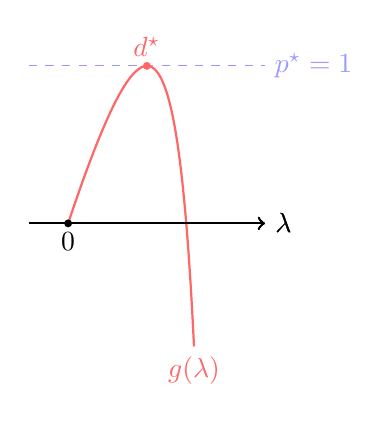
\begin{tikzpicture}[scale=2]
            \draw[smooth,thick,red!60,samples=100,variable=\l,domain=0:0.8] plot(\l,{4*\l - 1/(1-\l) + 1}) node[below]{$g(\lambda)$};
            \draw[thick,->] (-0.25,0) -- (1.25,0) node[right] {$\lambda$};
            \draw[thick,->] (-0.25,0) -- (1.25,0) node[right] {$\lambda$};
            \draw[blue!40,dashed] (-0.25,1) -- (1.25,1) node[right] {$p^\star=1$};
            \fill (0,0) circle (0.025) node[below] {$0$};
            \fill[red!60] (0.5,1) circle (0.025) node[above] {$d^\star$};
        \end{tikzpicture}
    \end{center}
    We can also see that $d^\star = 1 = p^\star$, satisfied by $\lambda^\star = 1/2$.
\end{example}

The above example exhibits no \emph{duality gap}: $p^\star - d^\star = 0$. In these situations, solving
the dual problem exactly gives us the optimal value of the primal problem. The situation that $d^\star = p^\star$
is known as \emph{strong duality}; the other case $d^\star < p^\star$ is known as \emph{weak duality}.
In the strong duality situation, using what's known as the KKT (Karush-Kuhn-Tucker) conditions, we can sometimes
easily recover the optimal parameters $\x^\star$ from this dual solution as well.

\subsection{Strong Duality and Slater's Condition}

As proposed above, strong duality can be an extremely helpful condition to exhibit, since it allows us to make
a choice of which optimization problem we want to solve to achieve at our solution. The question, then,
is if there are easy checks we can make to an optimization problem to see if strong duality holds. It turns
out that this is the case most of the time if our problem is convex.

An optimization problem is called \emph{convex} if it can be written in the form
\begin{align*}
    \text{minimize: } & f_0(\x)\\
    \text{subj. to: } & f_i(\x) \leq 0,\quad i=1,\ldots,m\\
                      & \A\x = \b
\end{align*}
where $f_i$ are all convex, $\A\in\R^{p\times n}$ and $\b\in\R^p$. This corresponds to
minimizing a convex function over a convex set.

\begin{theorem}[Slater's Condition]
    If our problem is convex and there exists an $\x\in \mathbf{dom} f_0$ so that
    \[
        f_i(\x) < 0,\,i=1,\ldots,m,\qquad\A\x=\b,
    \]
    then strong duality holds.
\end{theorem}

\subsection{Examples of Dual Problems (LP, QP)}

These will follow Boyd and Vandenberghe quite closely.

\begin{example}
    Consider the linear program
    \begin{align*}
        \text{minimize: } & \c^*\x\\
        \text{subj. to: } & \A\x = \b\\
                          & \x \geq 0.
    \end{align*}
    The Lagrangian is
    \[
        L(\x,\lambdab,\nub) = \c^*\x - \lambdab^*\x + \nub^*(\A\x - \b).
    \]
    For fixed $\lambda,\nu$, this is an affine function in $\x$ and hence we can find
    the dual function easily (verify this!)
    \[
        g(\lambdab,\nub) = \begin{cases}
            -\b^*\nub & \text{if } \A^*\nub - \lambdab + \c = 0\\
            -\infty   & \text{otherwise.}
        \end{cases}
    \]
    Such a $\lambdab\geq 0$ exists to satisfy the finite-dual condition
    $\A^*\nu = -\c + \lambdab$ so long as $\A^*\nu \geq -\c$. Since the non-negative
    multiplyer $\lambdab$ is not irrelevant to the dual function
    \[
        g(\lambdab,\nub) = \begin{cases}
            -\b^*\nub & \text{if }\A^*\nub \geq -\c\\
            -\infty &\text{otherwise,}
        \end{cases}
    \]
    we can write the dual problem to the original (primal) linear program above
    as
    \begin{align*}
        \text{minimize: } & \b^*\nub\\
        \text{subj. to: } & \A^*\nub \geq -\c,
    \end{align*}
    which is just another linear program. When does strong duality hold?
\end{example}

\begin{example}
    Suppose we have a matrix $\A\in\R^{n\times n}$ which is symmetric. We want to
    partition a group of items
    \[
        \{1,2,\ldots,n\} = \{i : \x_i = 1\} \cup \{i : \x_i = -1\} = A_+ \cup A_-
    \]
    into two sets $A_+$ and $A_-$, which are identified from a vector $\x\in\{\pm 1\}^n$.
    There is a profit $\A_{ij}$ associated with keeping $i$ and $j$ in the same partition,
    and a cost $-\A_{ij}$ associated with putting them in the same partition.
    Thus the total cost associated with a partition is (up to an addative constant $\tr\A$)
    equal to $\x^*\A\x$. We wish to find the partition which minimizes the cost. This
    corresponds to the optimization problem
    \begin{align*}
        \text{minimize: } & \x^*\A\x\\
        \text{subj. to: } & \x_i^2 = 1,\,i=1,2,\ldots,n.
    \end{align*}
    This problem is nonconvex and no apparent solution besides brute force iteration seems
    available, but passing to the dual (which turns out to be convex) allows us to efficiently
    find a lower bound to the problem. Exercise: prove $p^\star \leq \tr\A$.\\

    The Lagrangian
    \[
        L(\x,\nub) = \x^*\A\x + \sum_{i=1}^n \nub_i (\x_i^2 - 1) = \x^*(\A + \operatorname{diag}(\nub))\x - \boldsymbol{1}^*\nub.
    \]
    Thus the dual function
    \[
        g(\nub) = \inf_{\x} L(\x,\nub) = \begin{cases}
            -\boldsymbol{1}^*\nub & \text{if } \A + \operatorname{diag}(\nub) \succeq 0\\
            -\infty & \text{otherwise.}
        \end{cases}
    \]
    This gives the dual problem
    \begin{align*}
        \text{minimize: } & \boldsymbol{1}^* \nub\\
        \text{subj. to: } & \A + \operatorname{diag}(\nub) \succeq 0,
    \end{align*}
    which is a convex semidefinite program. It turns out strong duality does not hold here.
    Taking specific values of $\nub$ gives helpful lower bounds on the original problem without
    the need to solve exactly. For example, if $\nub = -\lambda_{\min}(\A)\boldsymbol{1}$ then
    \[
        \A + \operatorname{diag}(\nub) = \A - \lambda_{\min}(\A)\boldsymbol{1} \geq 0
    \]
    is dual feasible, and hence
    \[
        p^\star \geq -\boldsymbol{1}^*\nub = n\lambda_{\min}(\A).
    \]
    This bound is quite helpful when $\A$ is positive definite.
    In conclusion,
    \[
        n\lambda_{\min}(\A) \leq p^\star \leq \tr(\A).
    \]
\end{example}

\subsection{Application: Solutions to Linearly Constrained Quadratic Programs}

Consider the problem
\begin{align*}
    \text{minimize: } & \frac{1}{2}\x^*\Q\x + \c^*\x\\
    \text{subj. to: } & \A\x = \b\\
\end{align*}
where $\Q\in\R^{n\times n}$ is positive definite, $\c\in\R^n$, and $\A\in\R^{m\times n}, \b\in\R^m$.
For the optimal $\x$, $\A\x = \b$ by assumption. Moreovoer, strong duality holds
trivially if the problem is feasible, and so we can solve by the dual to find the original
problem. The Lagrangian
\[
    L(\x,\nub) = \frac{1}{2}\x^*\Q\x + \c^*\x + \nub^*(\A\x-\b),
\]
and for any $\nub$ the dual function must satisfy
\[
    \partial_{\x} L(\x,\nub) = \Q\x + \c + \A^*\nub = 0.
\]
Thus we have two equations
\[
    \A\x = \b,\quad \Q\x + \A^*\nub = -\c
\]
from which we can solve the primal and dual problem \emph{jointly} as the solution to
a single linear system
\[
    \m{\Q & \A^*\\\A & 0}\m{\x\\\nub} = \m{-\c\\\b}.
\]
This system is used heavily with interior point methods for solving arbitrary systems.

\subsection{Open Problem: Eigenvalues of Non-Negative Matrices via Convex Optimization}

If $\boldsymbol{A}\in\mathbb{R}^{n\times n}$ is positive and irreducible then the Collatz-Wielandt formula [AnantharamBorkar] says that the Perron-Frobenius eigenvalue
$$\lambda = \inf_{\boldsymbol{x} > 0} \max_{1\leq i \leq n} \frac{(\boldsymbol{Ax})_i}{\boldsymbol{x}_i}.$$
Write $\boldsymbol{z}\in\mathbb{R}^n$ as $\boldsymbol{z}_i = \log\boldsymbol{x}_i \in\mathbb{R}$ so that
$$\alpha := \log\lambda = \inf_{\boldsymbol{x} > 0} \max_{1\leq i \leq n} \log\frac{(\boldsymbol{Ax})_i}{\boldsymbol{x}_i} = \inf_{\boldsymbol{z}} \max_{1\leq i \leq n} \log\biggl(\sum_{j=1}^n\boldsymbol{a}_{ij}e^{\boldsymbol{z}_j}\biggr) - \boldsymbol{z}_i$$
since the logarithm is increasing and this transformation is a bijection. Here, $\boldsymbol{a}_i\in\mathbb{R}^n$ is the $i$-th row of $\boldsymbol{A}$. Define the function $f_i : \mathbb{R}^n \to \mathbb{R}$ by
\[
  f_i(\boldsymbol{z}) = \log\biggl(\sum_{j=1}^n\boldsymbol{a}_{ij}e^{\boldsymbol{z}_j}\biggr) - \boldsymbol{z}_i = \log\biggl(\sum_{j=1}^n e^{\boldsymbol{z}_j + \log \boldsymbol{a}_{ij}}\biggr) - \boldsymbol{z}_i.
\]
Convexity of the log-sum-exp function ensures that each $f_i$ are convex, and since the maximum
\[
f(\boldsymbol{z}) = \max_{1\leq i \leq n} f_i(\boldsymbol{z})
\]
of convex functions is convex we know that the problem of finding the log-Perron eigenvalue
\[
\alpha = \inf_{\boldsymbol{z}} f(\boldsymbol{z})
\]
is a convex optimization problem. Can we solve this optimization problem faster than the power
method, either in primal or dual form?

\end{document}
